\documentclass{ximera}

\title{This is the sample!}

\begin{document}

\begin{abstract}
Testing interactives and ff.
\end{abstract}

\maketitle

waffle and Jeff and fine.

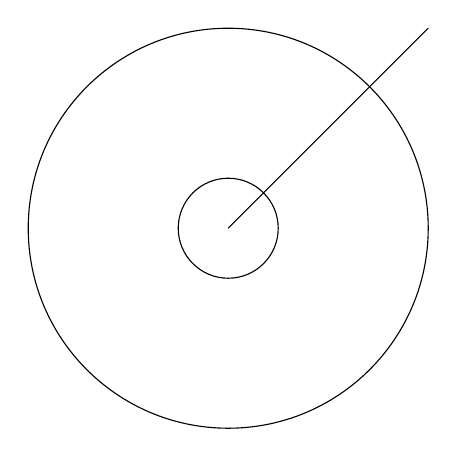
\begin{tikzpicture}
  \draw (0,0) circle (1in);
  \draw (0,0) circle (0.25in);
  \draw (0,0) -- (1in,1in);
\end{tikzpicture}

\begin{problem}
  String equality is like $\mbox{Dog} = \answer[format=string]{Dog}$.
\end{problem}

\begin{problem}
  The tolerance (0.01) means $8 \approx \answer[tolerance=0.01,id=y,format=integer]{8}$
  
  \begin{feedback}[72]
  \end{feedback}
\end{problem}

\begin{javascript}
x = 5;
\end{javascript}

And another one.  $x + 10 = \js{x+10}$ is equal to \js{x + 10}.

$\js{2+5} = 7$.

\end{document}
